\section{Quelques résultats utiles}

\paragraph{}
Les preuves ci-dessous ont été inspirées par~\cite{leemansTransactions}

\begin{lemma}
  Let $\Gamma$ be a "transitive" sggi over $n$ points such that the CPR graph have exactly $n-1$ edges. Then the CPR graph of $\Gamma$ is a string. %Transitive ??
\end{lemma}

\begin{proof}
  $\Gamma$ is transitive so its CPR graph is connex. And, because we have $n-1$ edges for $n$ vertices, the graph must be a tree.

  \paragraph{}
  Suppose now, that we have a vertex with at least three edges. Those edges are labelled with three differents numbers, $i, j, k$ that describe three different permutations, $\rho_i, \rho_j$ and $\rho_k$. But at least two of those permutations are not adjacent and so must not commute. We will consider that the involution $\rho_i$ and $\rho_k$ does not commute. %TODO Ref needed

  \paragraph{}
  And so by proposition 3.5 of~\cite{cprGraph}, the CPR graph where we only keep edge labelled with $i$ and $k$ must only contains those patterns:
  \begin{itemize}
    \item Fixed points
    \item Isolated edge (labelled with $i$ or $k$)
    \item Double edge
    \item Alternating square
  \end{itemize}
  But in our case, we already have two edges labelled $i$ and $k$ that connect the same point to two differents points. So the only way, we can extend this to a good pattern is with an alternating square. But we cannot have an alternating square because the graph is a tree and thus does not contains cycle.

  \paragraph{}
  So we cannot have vertex with three edges but the graph must be connex, so the only solution is a string.
\end{proof}

\begin{lemma}
  Let $\Gamma$ be a sggi avec $A_{11}$. Then $\Gamma$ contains at least two 4-transpositions if it's of rank 4 and at least one 4-transposition if its rank is 5.
\end{lemma}

\begin{proof}
  In both case, we have exactly 10 edges for 11 vertices. We can apply the previous lemma and so the CPR graph of $\Gamma$ is a string.

  \paragraph{Rank 5}
  The CPR graph is a string that contains exactly two edge for each of the five involutions. Because it's a string, each vertex must only be permuted by two adjacent permutations. For involution $\rho_0$, the two edges labelled with 0 can only be adjacent to the edges of $\rho_1$. But there are only two of them.
  Dans le cas du rang 5, s'il y avait uniquement des 2-transpositions alors il y aurait exactement 10 arêtes. Donc le graphe serait un chemin qui utiliserait exactement 2 arêtes pour chaque involution mais c'est impossible pour un rang impair. En effet, nous ne pouvons avoir d'arête double et donc, vu que nous devons utiliser exactement 2 fois chaque numéro, nous devons commencer par une arête $\rho_0$. En effet, sinon il faudrait plus de deux arêtes $\rho_1$. Il faut donc que le chemin commence et/ou se termine $\rho_0$. Par dualité, on a la même contrainte sur $\rho_3$ et donc une des deux involutions doit commencer le chemin tandis que l'autre doit le terminer. Celui-ci doit commencer comme ceci:

  \begin{figure}[H]
    \begin{center}
      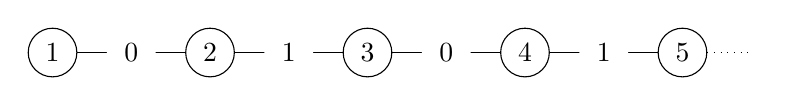
\begin{tikzpicture}

        \begin{scope}[every node/.style={circle,draw}]
          \node (1)  at (0,0)  {1};
          \node (2)  at (2,0)  {2};
          \node (3)  at (4,0)  {3};
          \node (4)  at (6,0)  {4};
          \node (5)  at (8,0)  {5};
        \end{scope}

        \node (6)  at (9,0) {};

        \begin{scope}[every node/.style={fill=white,circle}]

          \begin{scope}[every edge/.style={draw}]
            \path (1)  edge node {$0$} (2);
            \path (2)  edge node {$1$} (3);
            \path (3)  edge node {$0$} (4);
            \path (4)  edge node {$1$} (5);
            \path (5)  edge[style={dotted}] (6);
          \end{scope}
        \end{scope}



      \end{tikzpicture}
      \caption{}
    \end{center}
  \end{figure}

  \paragraph{}
  Une fois ce motif effectué, il faut obligatoirement continuer avec une arête $\rho_2$ et on est dans la même situation que précédement vu qu'il n'y a plus d'arête $\rho_0$ ou $\rho_1$. On rajoute toujours les arêtes par 4 et il est donc impossible d'arriver à 10 arêtes dans le cas du rang 5.

  \paragraph{Rang 4} Pour le rang 4, il nous faut au moins une 4-transposition pour arriver à 10 arêtes. Cette 4-transposition ne peut être $\rho_0$ car nous n'aurions pas assez d'arêtes de $\rho_1$ pour la relier. Il s'agit donc de $\rho_1$ (à la dualité près). Donc nous pouvons appliquer le même raisonnement que celui utilisé pour le rang 5 sur les involutions $\rho_2$ et $\rho_3$. Il faut donc que $\rho_3$ commence et/ou termine le chemin. S'il n'est utilisé qu'à une des deux extrémités, nous obtenons le début de chemin suivant:

  \begin{figure}[H]
    \begin{center}
      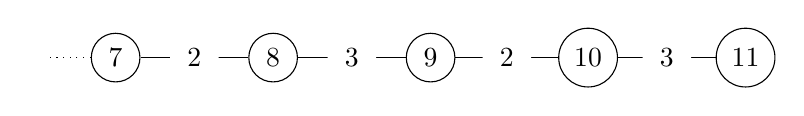
\begin{tikzpicture}

        \begin{scope}[every node/.style={circle,draw}]
          \node (5)  at (0,0)  {7};
          \node (4)  at (2,0)  {8};
          \node (3)  at (4,0)  {9};
          \node (2)  at (6,0)  {10};
          \node (1)  at (8,0)  {11};
        \end{scope}

        \node (6)  at (-1,0) {};

        \begin{scope}[every node/.style={fill=white,circle}]

          \begin{scope}[every edge/.style={draw}]
            \path (1)  edge node {$3$} (2);
            \path (2)  edge node {$2$} (3);
            \path (3)  edge node {$3$} (4);
            \path (4)  edge node {$2$} (5);
            \path (5)  edge[style={dotted}] (6);
          \end{scope}
        \end{scope}

      \end{tikzpicture}
      \caption{}
    \end{center}
  \end{figure}

\paragraph{}
Si nous voulons continuer le chemin, nous devons ajouter les arêtes suivante : $\rho_1, \rho_0, \rho_1, \rho_0, \rho_1$ mais il nous reste une arête $\rho_1$ à la fin. Il faudrait donc que $\rho_3$ commence et termine le graphe. On aurait un début de chemin comme suit:

\begin{figure}[H]
  \begin{center}
    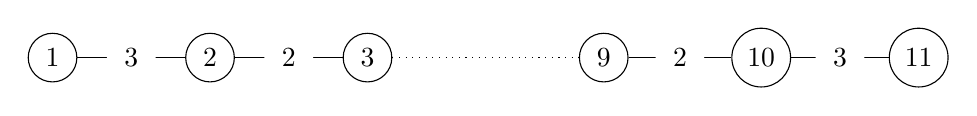
\begin{tikzpicture}

      \begin{scope}[every node/.style={circle,draw}]
        \node (1)  at (0,0)  {1};
        \node (2)  at (2,0)  {2};
        \node (3)  at (4,0)  {3};
        \node (9)  at (7,0)  {9};
        \node (10) at (9,0)  {10};
        \node (11) at (11,0) {11};
      \end{scope}



      \begin{scope}[every node/.style={fill=white,circle}]

        \begin{scope}[every edge/.style={draw}]
          \path (1)  edge node {$3$} (2);
          \path (2)  edge node {$2$} (3);
          \path (3)  edge[style={dotted}] (9);
          \path (9)  edge node {$2$} (10);
          \path (10) edge node {$3$} (11);
        \end{scope}
      \end{scope}

    \end{tikzpicture}
    \caption{}
  \end{center}
\end{figure}

\paragraph{}
Mais si on essaie de compléter les arêtes manquantes, on trouve qu'elle doivent commencer par $\rho_1, \rho_0, \rho_1, \rho_0, \rho_1$ car c'est la seule possibilité mais on ne sait pas placer la dernière arête $\rho_1$.

\end{proof}

\begin{lemma}
  Pour un sggi sur $A_{11}$, il n'est pas possible d'avoir deux 4-tranpositions non-adjacentes sauf s'il y a au moins une 4-transposition parmi les générateurs intermédiaires.
\end{lemma}

\begin{proof}
  Appelons les deux transpositions en question $\rho_i$ et $\rho_j$. Plaçons $\rho_i$ sur le graphe:

  \begin{figure}[H]
    \begin{center}
      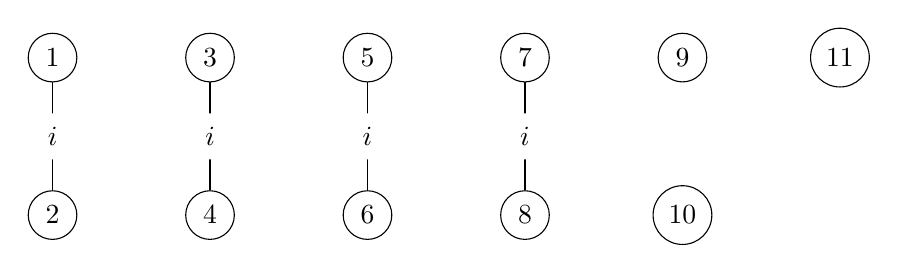
\begin{tikzpicture}

        \begin{scope}[every node/.style={circle,draw}]
          \node (1)  at (0,2)  {1};
          \node (2)  at (0,0)  {2};
          \node (3)  at (2,2)  {3};
          \node (4)  at (2,0)  {4};
          \node (5)  at (4,2)  {5};
          \node (6)  at (4,0)  {6};
          \node (7)  at (6,2)  {7};
          \node (8)  at (6,0)  {8};
          \node (9)  at (8,2)  {9};
          \node (10) at (8,0)  {10};
          \node (11) at (10,2) {11};
        \end{scope}

        \begin{scope}[every node/.style={fill=white,circle}]

          \begin{scope}[every edge/.style={draw}]
            \path (1)  edge node {$i$} (2);
            \path (3)  edge node {$i$} (4);
            \path (5)  edge node {$i$} (6);
            \path (7)  edge node {$i$} (8);
          \end{scope}
        \end{scope}

      \end{tikzpicture}
      \caption{Une seule 4-transposition $\rho_i$}
    \end{center}
  \end{figure}

  \paragraph{}
  Si nous voulons placer les arêtes de $\rho_j$ de telle sorte que $\rho_i$ commute avec $\rho_j$, alors, par la proposition 3.5 de~\cite{cprGraph} on doit utiliser une des trois solutions suivantes:
  \begin{enumerate}
    \item Doubler une arête de $\rho_i$
    \item Former un carré alterné avec $\rho_i$
    \item Relier deux points fixés par $\rho_i$.
  \end{enumerate}

  \paragraph{}
  Remarquons que le fait de relier deux points fixés par $\rho_i$ ne peut être utilisé que pour placer une des quatre arêtes de $\rho_j$. Donc nous devons trouver une solution pour au moins les trois restantes. Nous avons donc les possibilités suivantes:
  \begin{enumerate}
    \item Deux carrés alternés
    \item Un carré alterné, une arête doublée et une arête reliant des points fixes
    \item Un carré alterné et deux arête doublées
    \item Trois arêtes doublées et une arête reliant deux points fixes
    \item Quatre arêtes doublées.
  \end{enumerate}

  \paragraph{}
  Nous allons traiter les cas un par un

  \paragraph{Deux carrés alternés}
  Dessinons le graphe CPR de ce cas

  \begin{figure}[H]
    \begin{center}
      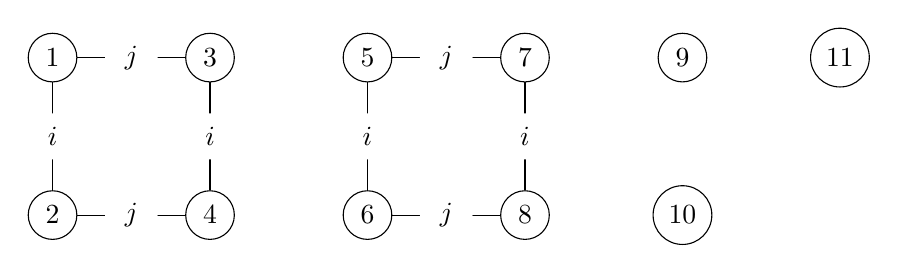
\begin{tikzpicture}

        \begin{scope}[every node/.style={circle,draw}]
          \node (1)  at (0,2)  {1};
          \node (2)  at (0,0)  {2};
          \node (3)  at (2,2)  {3};
          \node (4)  at (2,0)  {4};
          \node (5)  at (4,2)  {5};
          \node (6)  at (4,0)  {6};
          \node (7)  at (6,2)  {7};
          \node (8)  at (6,0)  {8};
          \node (9)  at (8,2)  {9};
          \node (10) at (8,0)  {10};
          \node (11) at (10,2) {11};
        \end{scope}

        \begin{scope}[every node/.style={fill=white,circle}]

          \begin{scope}[every edge/.style={draw}]
            \path (1)  edge node {$i$} (2);
            \path (3)  edge node {$i$} (4);
            \path (5)  edge node {$i$} (6);
            \path (7)  edge node {$i$} (8);
            \path (1)  edge node {$j$} (3);
            \path (2)  edge node {$j$} (4);
            \path (5)  edge node {$j$} (7);
            \path (6)  edge node {$j$} (8);
          \end{scope}
        \end{scope}

      \end{tikzpicture}
      \caption{Deux 4-transpositions formant deux carrés alternés}
    \end{center}
  \end{figure}



\end{proof}
